\documentclass[a4paper,14pt]{extarticle}
\usepackage[utf8]{inputenc}
\usepackage[russian]{babel}
\usepackage{graphicx}
\usepackage[top=0.8in, bottom=0.8in, left=0.8in, right=0.8in]{geometry}
\usepackage{pgfplots}
\usepackage{amsmath}
\usepackage{setspace}
\usepackage{titlesec}
\usepackage{float}
\usepackage{chngcntr}
\usepackage{pgfplots}
\usepackage{amsfonts}
\usepackage{pgfplotstable}
\usepackage{multirow}
\usepackage{karnaugh-map}
\usepackage{tikz,xcolor}
\usepackage{listings}

\titleformat{\section}[hang]
  {\bfseries}
  {}
  {0em}
  {\hspace{-0.4pt}\large \thesection\hspace{0.6em}}
  
  
\titleformat{\subsection}[hang]
  {\bfseries}
  {}
  {0em}
  {\hspace{-0.4pt}\large \thesubsection\hspace{0.6em}}
  
\newcommand{\nx}{\overline{x}}
\newcommand{\p}{0.31}
\newcommand{\scale}{1.4}

\counterwithin{figure}{section}
\counterwithin{equation}{section}
\counterwithin{table}{section}

\lstdefinestyle{CStyle}{
    basicstyle=\footnotesize,
    breakatwhitespace=false,         
    breaklines=true,                 
    captionpos=b,                    
    keepspaces=true,                 
    numbers=left,                    
    numbersep=5pt,                  
    showspaces=false,                
    showstringspaces=false,
    showtabs=false,                  
    tabsize=2,
    language=C
}

\begin{document}
\begin{titlepage}
\centering
\small Балтийский государственный технический университет «Военмех» им. Д.Ф.Устинова \\
\vspace{3cm}
\normalsize Кафедра И5\\
«Информационные системы и программная инженерия»\\
\vspace{3cm}
\textbf{Практическое задание №4}\\
по дисциплине Основы программирования на тему\\ 
\textbf{«Массивы. Динамическое выделение памяти»}\\
Вариант 14
\vfill

\begin{flushleft}
\textbf{Выполнил:}
\hfill {Мальцев А.С.} \\
\hfill {Группа И595} \\
\vspace{1cm}
\textbf{Преподаватель:}
\hfill {Лазарева Т.И.} \\
\end{flushleft}
\vspace{3cm}

{\centering Санкт-Петербург \\ 
\vspace{0.15cm}
2019}
\end{titlepage}
\setcounter{page}{2}
\section{Цель работы}
Ознакомиться с организацией массивов в языке Си, изучить принципы работы с массивами,освоить работу с массивами через указатели, научиться грамотно выделять и освобождать память в процессе работы программы.

\section{Ход работы}
\subsection{Задание 1}
Вычислить среднее арифметическое значение элементов массива А (7), не встречающихся в массиве В (5).\\
\textit{Исходные данные:} входные значения могут быть любыми, поэтому a и b типа double.\\
\textit{Результирующие данные:} т.к. a и b - типа double, а так же при нахождении среднего арифметического требуется операция деления, то s - типа double.
\begin{center}
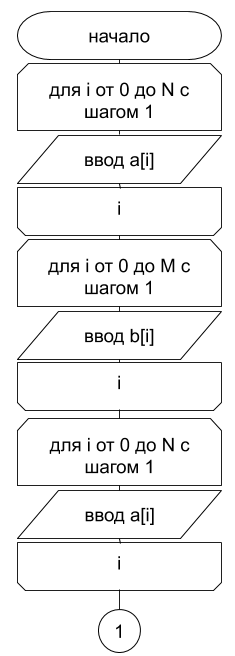
\includegraphics[scale=0.6]{lab4-1-1.png}\\
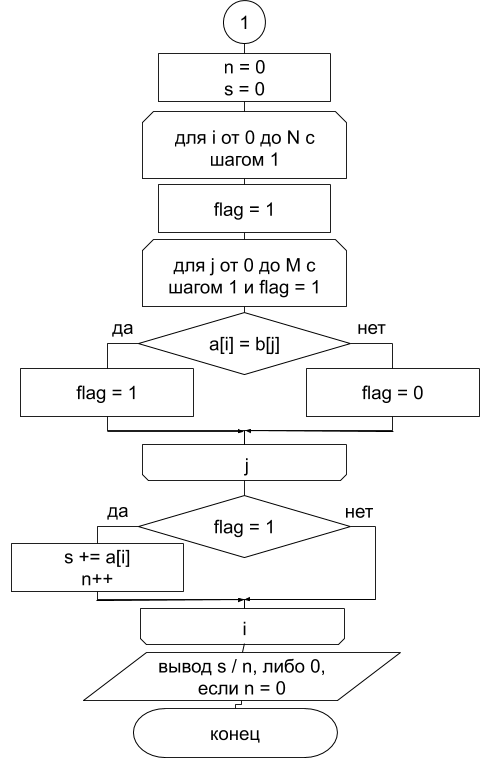
\includegraphics[scale=0.6]{lab4-1-2.png}\\
Схема программы
\end{center}
\lstinputlisting[language=c, frame=single, style=CStyle]{../1.c}
\begin{center}
Текст программы\\
\vspace{0.6cm}
\begin{tabular}{|l|l|}
\hline
\multicolumn{1}{|c|}{Исходные данные}& \multicolumn{1}{|c|}{Вывод программы}\\
\hline
a = 1 2 3 4 5 6 7 & s = 2.500000 \\
b = 5 6 7 10 8 & \\
\hline
a = 1 2 3 4 5 1 2 & s = 0.000000 \\
b = 1 2 3 4 5 & \\ 
\hline
\end{tabular}\\
\vspace{0.3cm}
Результаты тестирования
\end{center}

\subsection{Задание 2}
Найти наименьший положительный элемент линейного массива, значение которого принадлежит диапазону [ X , Y ], и удалить его, сдвинув оставшиеся элементы к началу массива. Отрицательное или нулевое значение Y является некорректным. Если в массиве нет элементов, значения которых лежат в диапазоне [ X , Y ], вывести сообщение об этом. Если найдется несколько элементов, удовлетворяющихпоставленным условиям, удалить первый из них.\\
\textit{Исходные данные:} входные значения могут быть любыми, поэтому a, x и y типа double. n - количество элементов в массиве, целое число.\\
\textit{Результирующие данные:} результатом работы будет измененный массив a.\\
\begin{center}
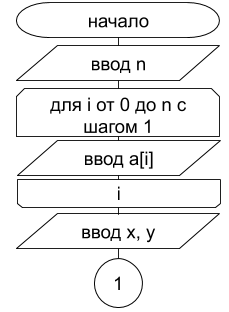
\includegraphics[scale=0.6]{lab4-2-1.png}\\
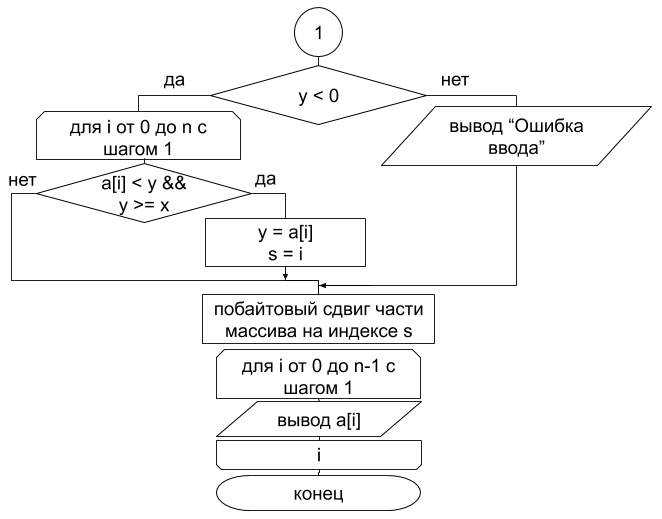
\includegraphics[scale=0.6]{lab4-2-2.png}\\
Схема программы
\end{center}
\lstinputlisting[language=c, frame=single, style=CStyle]{../2.c}
\begin{center}
Текст программы\\
\vspace{0.6cm}
\begin{tabular}{|l|l|}
\hline
\multicolumn{1}{|c|}{Исходные данные}& \multicolumn{1}{|c|}{Вывод программы}\\
\hline
n = 5, x = 3, y = 5 & a = 1.000000 2.000000 4.000000 5.000000 \\
a = 1 2 3 4 5 & \\
\hline
n = 7, x = 1, y = 5 & a = 7.000000 3.000000 8.000000 3.000000 6.000000 5.000000  \\
a = 3 7 3 8 3 6 5 & \\
\hline
\end{tabular}\\
\vspace{0.3cm}
Результаты тестирования
\end{center}

\subsection{Задание 3}
Отсортировать каждую строку матрицы А (3х3) в порядке убывания.\\
\textit{Исходные данные:} входные значения могут быть любыми, поэтому матрица a типа double.\\
\textit{Результирующие данные:} результатом работы будет отсортированная матрица a.\\
\begin{center}
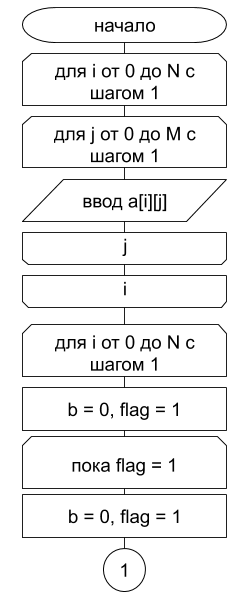
\includegraphics[scale=0.6]{lab4-3-1.png}\\
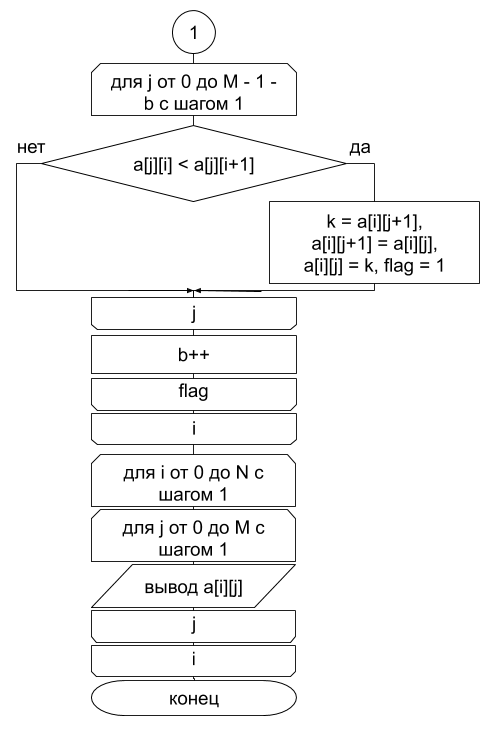
\includegraphics[scale=0.6]{lab4-3-2.png}\\
Схема программы
\end{center}
\lstinputlisting[language=c, frame=single, style=CStyle]{../3.c}
\begin{center}
Текст программы\\
\vspace{0.6cm}
\begin{tabular}{|l|l|}
\hline
\multicolumn{1}{|c|}{Исходные данные}& \multicolumn{1}{|c|}{Вывод программы}\\
\hline
1 2 3 & 3 2 1\\
4 5 6 & 6 5 4\\
7 8 9 & 9 8 7\\
\hline
4 8 22 & 22 8 4\\
5 9 55 & 55 9 5\\
0 -4 8 & 8 0 -4\\
\hline
\end{tabular}\\
\vspace{0.3cm}
Результаты тестирования
\end{center}

\subsection{Задание 4}
Определить, является ли данная целочисленная квадратная матрица симметричной относительно своей главной диагонали.\\
\textit{Исходные данные:} входные значения могут быть любыми, поэтому матрица a типа double. n - порядок матрицы, целое значение.\\
\textit{Результирующие данные:} для вывода результата дополнительной переменной не требуется.\\
\textit{Дополнительные переменные:} вспомогательная перменная isSym для того, чтобы запомнить, симметрична ли матрица.\\
\begin{center}
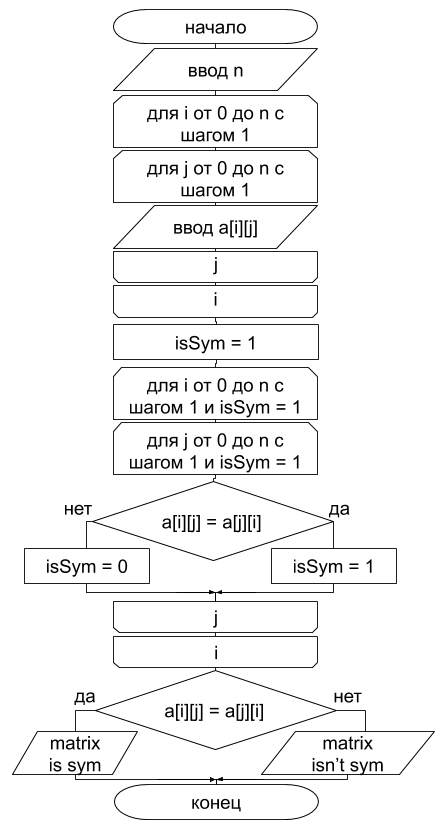
\includegraphics[scale=0.6]{lab4-4.png}\\
Схема программы
\end{center}
\lstinputlisting[language=c, frame=single, style=CStyle]{../4.c}
\begin{center}
Текст программы с использованием статического массива\\
\end{center}
\lstinputlisting[language=c, frame=single, style=CStyle]{../4-d.c}
\begin{center}
Текст программы с использованием динамического массива\\
\vspace{0.6cm}
\begin{tabular}{|l|l|}
\hline
\multicolumn{1}{|c|}{Исходные данные}& \multicolumn{1}{|c|}{Вывод программы}\\
\hline
4 & matrix is sym \\
1 2 3 4 & \\
2 3 4 5 & \\
3 4 5 6 & \\
4 5 6 7 & \\
\hline
3 & matrix isn't sym \\
3 3 3 & \\
7 4 0 & \\      
-99 5.567 999999 & \\
\hline
\end{tabular}\\
\vspace{0.3cm}
Результаты тестирования
\end{center}

\subsection{Задание 5}
Детские пластиковые кубики трех цветов сложены в прямоугольный параллелепипед размером M x N x P кубиков. Определить, найдется ли в этом параллелепипеде хотя бы один слой толщиной в один кубик, расположенный параллельно какой-нибудь грани параллелепипеда и сложенный из кубиков одного цвета.\\
\textit{Исходные данные:} входные значения могут быть любыми, поэтому матрица cont типа double. m, n, p - размерности трехмерного массива, целые значения.\\
\textit{Результирующие данные:} для вывода результата дополнительной переменной не требуется.\\
\textit{Дополнительные переменные:} вспомогательная перменная sFlag для того, чтобы запомнить, найден ли был слой из одинаковых кубиков.\\
\begin{center}
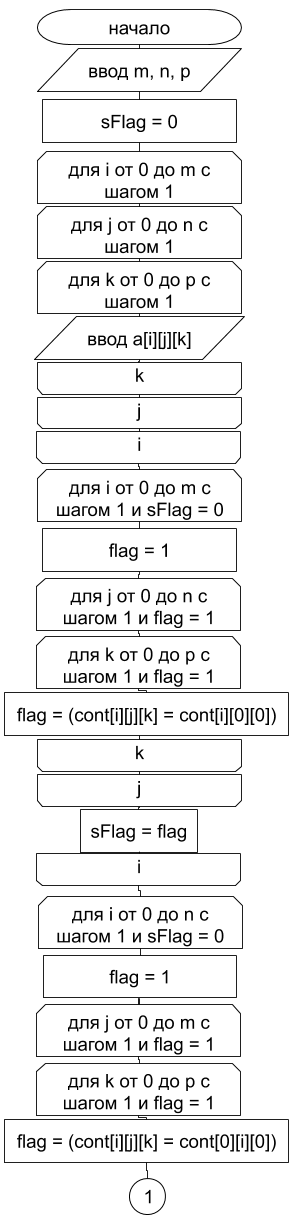
\includegraphics[scale=0.6]{lab4-5-1.png}\\
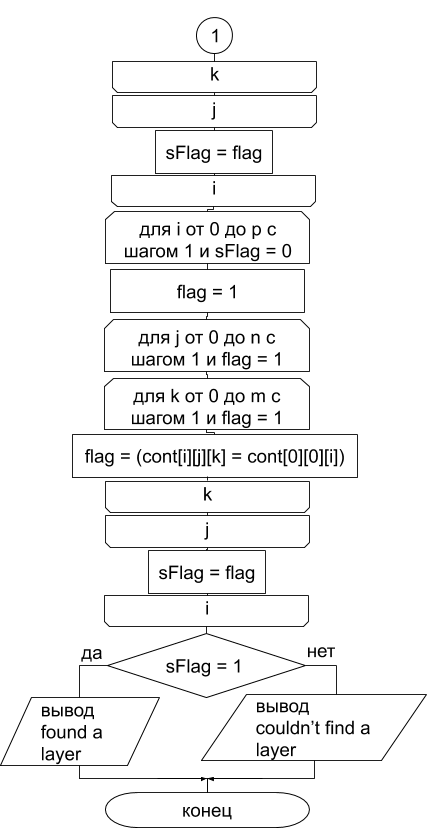
\includegraphics[scale=0.6]{lab4-5-2.png}\\
Схема программы
\end{center}
\lstinputlisting[language=c, frame=single, style=CStyle]{../5.c}
\begin{center}
Текст программы\\
\vspace{0.6cm}
\begin{tabular}{|l|l|}
\hline
\multicolumn{1}{|c|}{Исходные данные}& \multicolumn{1}{|c|}{Вывод программы}\\
\hline
3 3 3 & found a layer \\
2 6 8 | 3 0 0 | 4 8 9 & \\
5 5 5 | 5 5 5 | 5 5 5 & \\
6 8 9 | 3 0 4 | 3 1 7 & \\
\hline
2 2 3 & couldn't find a layer \\
1 4 | 2 7 | 1 6 & \\
7 8 | 9 0 | 2 8 & \\
\hline
\end{tabular}\\
\vspace{0.3cm}
Результаты тестирования
\end{center}


\end{document}
